\documentclass[../Elmag-labhefte-2020.tex]{subfiles}

\begin{document}


\setchapterpreamble[u]{\margintoc}
\chapter{Force on a conductor\label{ch.kraft}}

\subsection*{Goal}

In this lab assignment you will
%
\begin{itemize}
\item develop your skills in documenting laboratory work in the lab journal,
\item study the force between a live conductor and a constant magnetic field,
\item gain experience in producing results from precision measurements,
\item perform data processing of the measurement results using regression analysis in Python (method of least squares). % og/eller Excel
\end{itemize}
%


%**********************************************
\section{Theoretical background}
%**********************************************

%Teorien presenteres i samband med beregningsoppgavene nedenfor. Forøvrig vises til lærebok og forelesningene i elektromagnetisme.


%%%%%%%%%%%%%%%%%%%%%%%%%%%%%%%%%%%%%%%%%%%%%%%%%%%
%\section{Beregningsoppgaver \label{ch.kraft.beregn}}
%%%%%%%%%%%%%%%%%%%%%%%%%%%%%

\subsection{Force on a conductor \label{ch.kraft.beregn1}}
%%%%%%%%%%%%%%%%%%%%%%%%%%%%%
An electron with charge $q = -e$ moving at a speed $\va*{v}$ in a conductor located in a magnetic field $\va*{B}$ will be affected by a force according to the Lorentz force
\begin{equation}
    \va*{F} = q \va*{v} \cross \va*{B}.
\end{equation}
%
 The total force on a live conductor in a magnetic field is the total force on all the electrons in the conductor:
\begin{equation}
    \va*{F} = q (\va*{v}_d \cross \va*{B} ) n A \ell,
\end{equation}
%
where $\ell$ is the length of the conductor, $A$ is the cross-sectional area, $n$ is the electron density and consequently $n A \ell$ is equal to the total number of electrons in the conductor. The speed $\va*{v}_d$ must be understood as the average velocity (drift velocity) of the electrons.
The electric current in a conductor is defined as
\begin{equation}
    I = nqv_d A ,
\end{equation}
and consequently the force can be expressed
\begin{equation}
    \va*{F} = I\va*{\ell} \cross \va*{B},
\end{equation}
%
where $\va*{\ell}$ is understood as the vector with direction along the conductor in the current direction, with length \(l\). In scalar quantities, the equation is
\begin{equation}
    F = I\ell B \sin \theta,
    \label{eq:kraft.5}
\end{equation}
where $\theta$ is the angle between the magnetic field and the positive current direction in the conductor.
When the conduction direction is perpendicular to the magnetic field $\theta = \pi/2$, and equation \eqref{eq:kraft.5} is simplified to
\begin{equation}
    F = I\ell B.
    \label{eq:kraft.6}
\end{equation}
%
The force on a live conductor in a magnetic field can be measured with the arrangement in Figure \ref{kraft.fig1}.
\begin{figure}[htb]
    \centering
    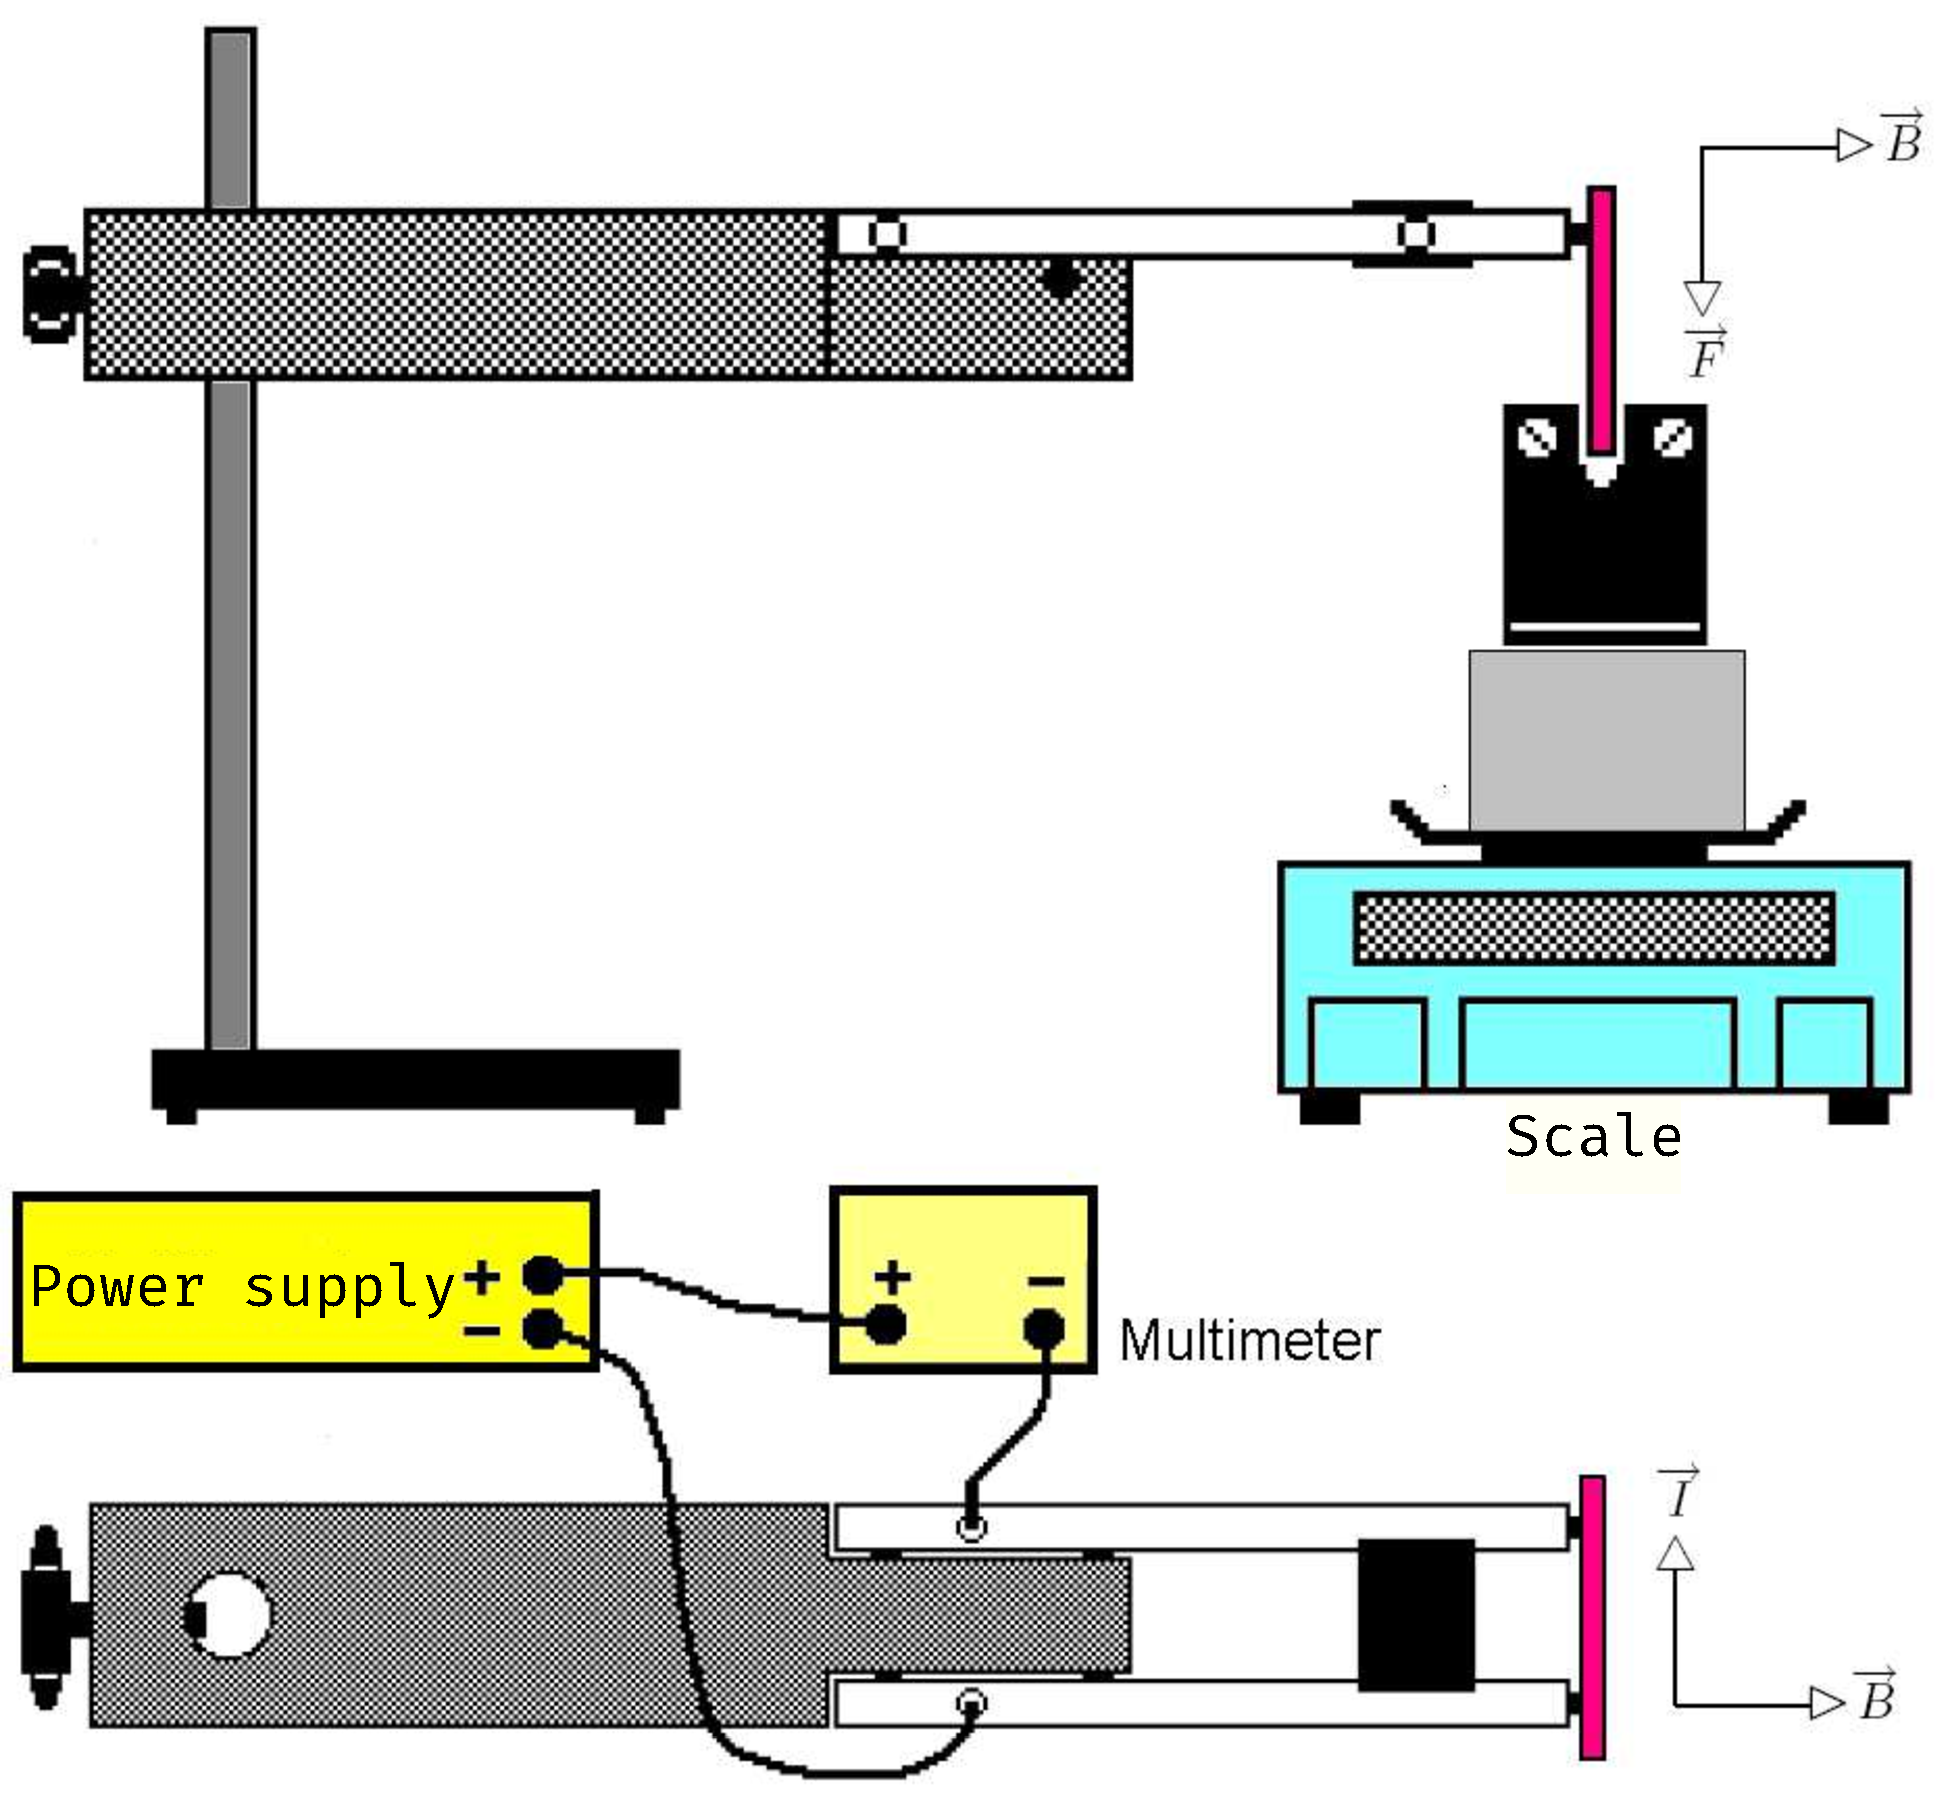
\includegraphics[width=0.75\textwidth]{KraftFig1_english}
    \caption{%
        Sketch of the setup used for measuring force on a live conductor.
        \textbf{(Top)} Seen from the side.
        \textbf{(Bottom)} Seen from above.
    }
    \label{kraft.fig1}
\end{figure}
The magnet rests on the scale, while the live conductor is fixed independently of the scale. The force between the conductor and the magnet will be registered on the scale. However, the weight is calibrated and graded to measure mass $M$ in grams as a certain value for gravitational acceleration $g$ is assumed. As is well known, the connection between power and mass is given by
\begin{equation}
    F = M g, 
    \label{eq:kraft.7}
\end{equation}
so that from equation \eqref{eq:kraft.5} we will express the mass reading on the scale as:
\begin{equation}
    M = \frac{I \ell B}{g} \sin \theta.
    \label{eq:kraft.8}
\end{equation}
%Når $\theta = \pi/2$, kan likning \eqref{eq:kraft.8} omskrives som
%\begin{equation}
%    M (I) = a_1^\prime I,
%    \quad \bigl 
%    (a_1^\prime = \ell B/g \bigr),
%    \label{eq:kraft.8a}
%\end{equation}
%eller som
%\begin{equation}
%    M(\ell) = b_1^\prime \ell,
%    \quad \bigl 
%    ( b_1^\prime = IB/g\bigr ).
%    \label{eq:kraft.8b}
%\end{equation}

%\subsection{Kraft sfa. strøm og lederlengde \label{ch.kraft.beregn2}}
%%%%%%%%%%%%%%%%%%%%%%%%%%%%%

%{\emph 1. Bruk Excel eller MATLAB til å sette opp et kurvediagram over vekta $M$ i gram som funksjon av trådlengden $\ell$ langs $x$-aksen i området 0 til 100 mm når du antar $B$ = 700 gauss. Lag fem kurver i diagrammet der strømmen er parameter: $I = $ 1, 2, 3, 4 og 5 A.
%}

%Bruk likning (\ref{eq:kraft.8}) med $\sin \theta = 1$ og $g = 9,82 \times 10^{-3} $ N/g. 


%\textbf{2. Sett opp et annet kurvediagram med samme størrelse langs $y$-aksen men med strømmen $I$ i området 0 til 5 A langs $x$-aksen. Lag fire kurver med lengden av tråden som parameter: $\ell = $ 12,5; 22,5; 32,5 og 42 mm.} 

\subsection{Force as a function of angle \label{ch.kraft.beregn3}}
%%%%%%%%%%%%%%%%%%%%%%%%%%%%%

\begin{marginfigure}%[h]
    \setlength{\unitlength}{1mm}
    % \fbox{ % For showing the boundig box of figure
      \begin{picture}(60,50)(15,0)
        % \multiput(30,12.5)(6,6){3}{\line(1,1){5}} 
        \multiput(30.3,12.3)(0.75,0.75){26}{$\cdot$} %\multiput(30,12.5)(0.75,0.75){26}{\circle{0.5}}
        
        \linethickness{0.2mm}
        \newsavebox{\dumb}
        \savebox{\dumb}(10,10)[l]{
          \put(28,-20){\line(-3,2){18}} %\put(10,10){\line(1,-2){15}} 
          \put(27.4,-20.8){\tiny$\otimes$}%\put(28,-20){\circle}
          % \put(10,-8){\circle{1.59}} %\put(10,-8){\circle{1.59}} 
          % \put(9.5,-9){$\cdot$}
          % \put(27.1,-20.5){\small$\times$}
          \put(8.7,-8.2){\tiny$\odot$}
        } 
        \multiput(20,20)(1.2,1.2){10}{\usebox{\dumb}} 
        \qbezier(32,48)(28,43)(31,39)
        \put(30.5,36.5){$\searrow$}
        \thicklines
        \put(26,15){\line(0,1){30}} 
        \put(26,15){\line(-1,0){10}} 
        \put(26,45){\line(-1,0){10}} 
        
        
        \put(51,33.3){\vector(-3,2){9.6}}%11 mm arrow northwest
        \put(51,33.3){\vector(3,-2){9}}%11 mm arrow southeast
        \put(35,35.5){\vector(1,1){4.5}}
        \put(35,35.5){\vector(-1,-1){6.5}}
        % \color{black}
        \put(32,48){10 windings}
        
        
        \put(62,15){\line(0,1){30}} 
        \put(62,15){\line(1,0){10}} 
        \put(62,45){\line(1,0){10}} 
        
        \put(18,28){\huge N}
        \put(68,28){\huge S}
        
        \put(50,35){$\swarrow$}
        \put(48,41){$\underbrace{\;11 \mbox{mm}\;}$}
        
        \put(30,12.5){\vector(1,0){20}} %B-vector
        \put(30,12.5){\vector(3,-2){15}} %I-vector
        \qbezier(40,12.5)(41,10)(39,7) %Arc for theta
        % 
        
        % \put(30,12.5){\line(1,1){20}} 
        
        \put(51,11){$\va*{B}$}
        \put(46,3){$\va*{I}$}
        \put(41,8){$\theta$}
      \end{picture}
      % } % fbox
    \caption{%
        Turnable coil placed in the magnetic well, seen from above.
        Only the lower part of the coil is in the magnetic field.
        The vertical conductors (marked with \(\otimes\) and \(\odot\)) experience horizontal forces, which in total zero out.
    }
    \label{kraft.fig2}
\end{marginfigure}

You replace the conductor with a coil as shown in Figure \ref{kraft.fig2} where the angle between the coil axis and the magnetic field direction is variable. The coil has $N = 10$ rectangular windings with side lengths \SI{11}{\mm} and only the lower part of the coil lies in the magnetic field so that the force only acts on the lower horizontal part of the windings, i.e. a total length of \SI{110}{\mm}. The angle between the current direction and the magnetic field is $\theta$ and is included in the equation for calculating the force.


%\begin{figure}[h]
%\begin{center}
%\vspace{1cm}
%\hspace{-4cm}
%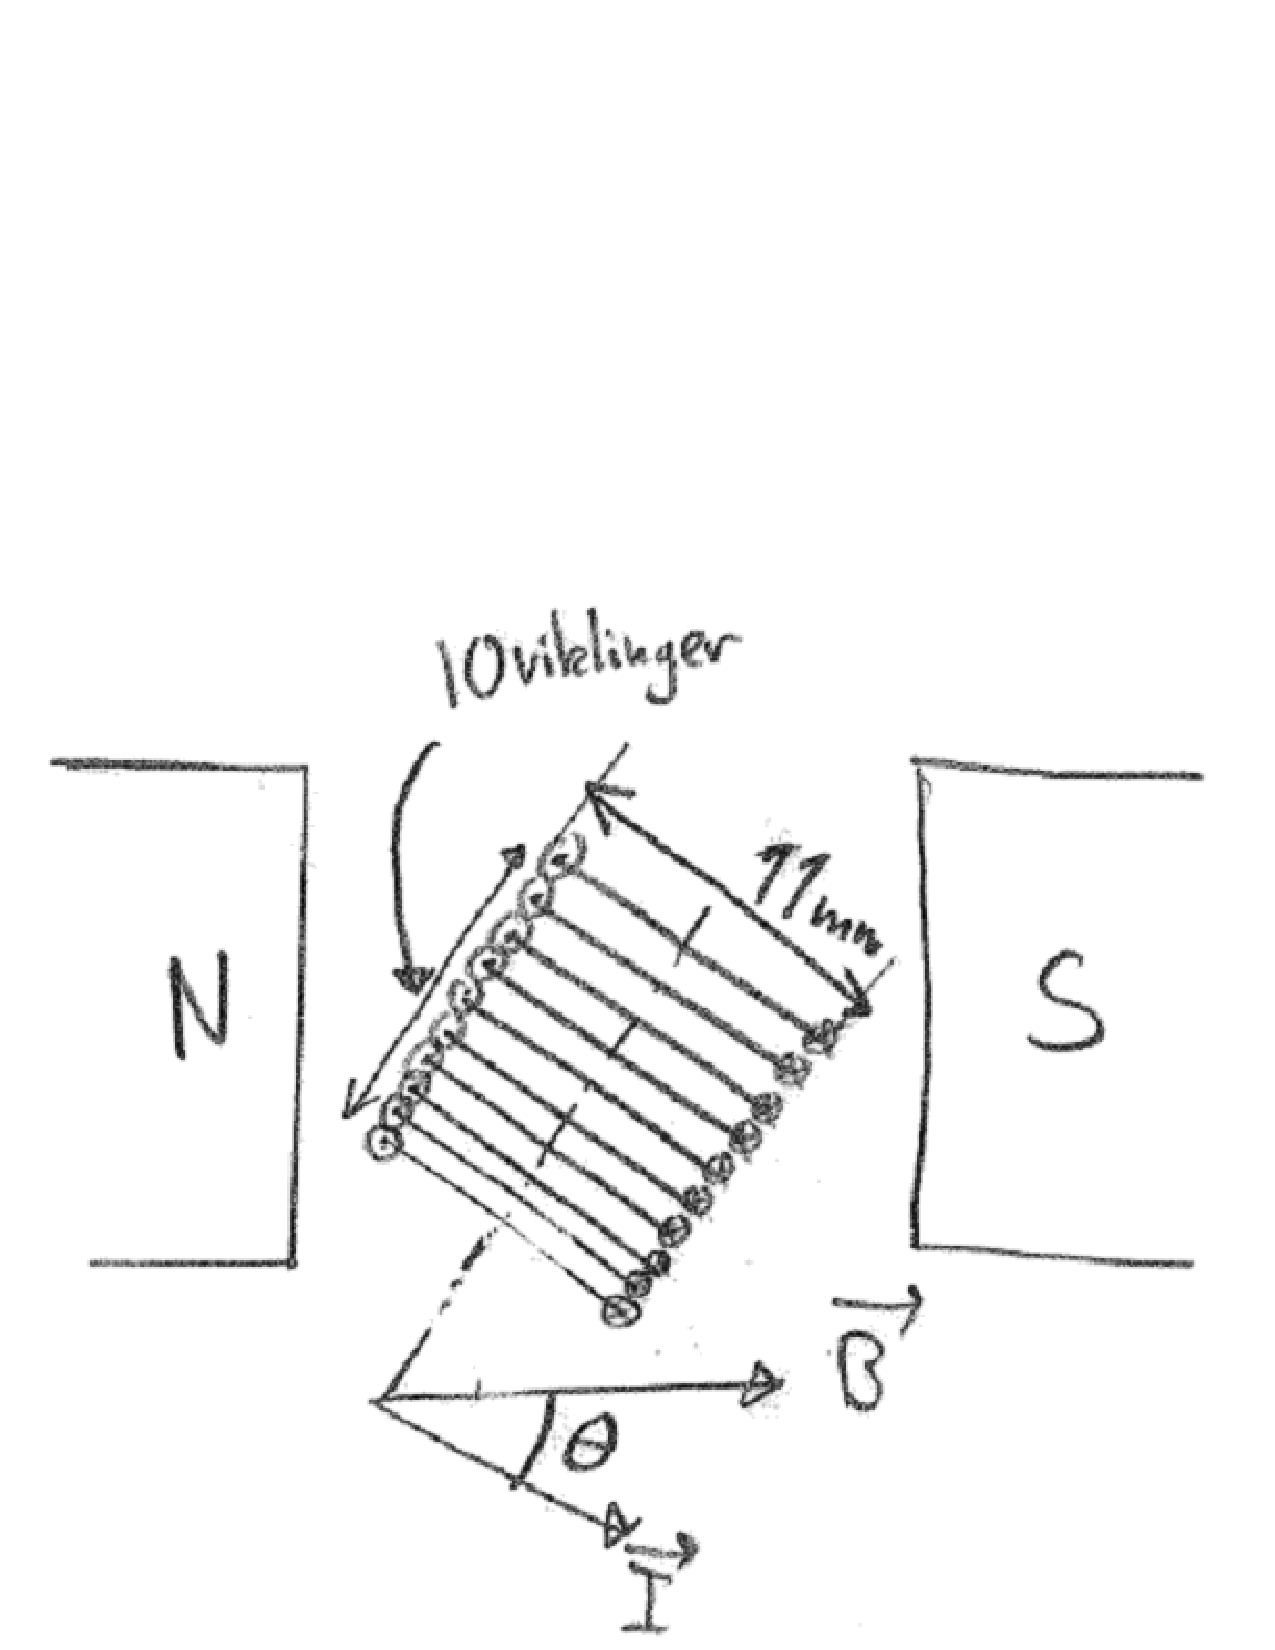
\includegraphics[bb=0 0 450 412,width=6cm,height=9cm,keepaspectratio]{KraftFig2}
%\vspace{-8mm}
%\end{center}
%\caption{\sf Dreibar spole plassert i magnetbrønnen, sett ovenfra. Kun den nedre delen av spolen ligger i magnetfeltet og de vertikale lederne (markert med $\times$ og $\cdot$ på figuren) er påvirket av krefter i horisontal retning og som innbyrdes nuller hverandre ut.}
%\label{kraft.fig2}
%\end{figure}


%{\emph 2. Bruk Excel eller MATLAB til å sette opp et kurvediagram over vekta $M$ i gram som funksjon av vinkelen $\theta$ i grader i området -90$^\circ$ til +90$^\circ$. Lag to kurver i diagrammet med strømmen som parameter: $I = $ 2 og 4 A. Bruk trådlengde 11 mm $\times$ 10 = 110 mm og  $B$ = 200 gauss.
%}

%\subsection{Elektrisk motor  \label{ch.kraft.beregn4}}
%%%%%%%%%%%%%%%%%%%%%%%%%%%%%

%}


\section{Preliminary Tasks}
Familiarize yourself with the linear curve fitting script located on the Blackboard (Jupyter notebook). Two examples of data sets that can be used for testing are distributed.

%%%%%%%%%%%%%%%%%%%%%%%%%%%%%%%%%%%%%%%%%%%%%%%%%%%%%%%%%%%%%%%%%%%%%%%%%%%%%%
\section{Experimental \label{ch.kraft.eksp}}
%%%%%%%%%%%%%%%%%%%%%%%%%%%%%%%%%%%%%%%%%%%%%%%%%%%%%%%%%%%%%%%%%%%%%%%%%%%%%%

%%%%%%%%%%%%%%%%%%%%%%%%%%%%%%%%%%%%%%%%%%%%%%%%%%%%%%%%%%%%%%%%%%%%%%%%%%%%%%
\subsection{Equipment}
%%%%%%%%%%%%%%%%%%%%%%%%%%%%%%%%%%%%%%%%%%%%%%%%%%%%%%%%%%%%%%%%%%%%%%%%%%%%%%

The following instruments are included in the line-up:
\vspace{-4mm}
\begin{itemize}
    \item \textbf{Electromagnetic scale.} Mettler Mod. PM480. Range: 0- \SI{400}{\g}. Precision: $\pm \SI{1}{\milli\g}$, or Mettler Mod. PB-SDR / FACT. Range 0- \SI{60}{\g} $\pm$ \SI{1}{\milli\g} / 70- \SI{310}{\g} $\pm$ \SI{8}{\milli\g}.
    \item \textbf{Mount.} Pasco SF-8607.
    \item \textbf{Solid conductors} and \textbf{magnetic well} with variable magnetic field from \SI{125}{\G} to \SI{750}{\G} in steps of \SI{125}{\G}. Make and type: Pasco SF-8607. Max 5A
    \item \textbf{Turnable coil} with 10 rectangular windings horizontal, dimension 11 $\times$ \SI{23}{\mm}, with associated magnetic well with magnetic field equal to approx. \SI{250}{\G}. Max 5A.
    Make and type: Pasco SF-8608.
    \item \textbf{Power supply.} Fredriksen Mod. 364000. Area: 0- \SI{24}{\volt} 0- \SI{10}{\ampere}. Used as a power source.
    \item \textbf{Multimeter.} Keithley 175A or GW plug GDM-8246.
    \item \textbf{Gaussmeter.} Magnetic Instruments RFL, Mod. 912. \\
    Measuring range: \(\SI{0.01}{\G} - \SI{100}{\kilo\G} \). Catalog \\
    Precision: \(\pm \) (0.4 \% of reading + 0.1 \% of range + 1 in the last digit).\\
    Transversal probe.
    \item \textbf{Calipers.}
\end{itemize}

The scale is a precision instrument that you must handle with care.
Take special care to avoid impacts to the scale's bottom plate during assembly and disassembly of the setup. The scale is based on an electromagnetic weighing method according to the compensation principle so that the bottom plate does not change position during weighing. This is important for our measurements.

%Figuren til venstre viser vektas oppbygging skjematisk: En spole er viklet på veiepannen. Spolen er senket ned i en sirkulær permanent magnetbrønn som gir et konstant magnetfelt.  Når veiepanna blir belastet genereres det en strøm i spolen som i vekselvirkning med magnetfeltet gir en kraft som kompenserer for bevegelsen av veiepannen. Veiepannens posisjon blir overvåket av en optisk sensor som er koplet i en servosløyfe som regulerer strømmen i spolen slik at posisjonen ikke forandres.

The conductors used in the experiments are built up as modern electronic circuit boards with narrow current paths of copper mounted on fiberglass-reinforced polyester sheets. To prevent oxidation of the copper surface, it is covered with tin. In total, the instrument set-up contains six fixed current paths of different lengths, of which four are single and two are double.

As a magnetic field source, a magnetic well built up of six identical permanent magnets is used. The field in the well can be varied by removing the magnets one by one.

To investigate the power as a function of the angle between field direction and current direction the last experiment utilizes a rotatable coil with its own magnetic well.



\subsection{Force as a function of the current}
%%%%%%%%%%%%%%%%%%%%%%%%%%%%%%%%%%%%%

Task:
\emph{Investigate how the force between a thin conductor and a magnetic field normal to the conductor depends on the current in the conductor.}

Suggested procedure:
%
\begin{itemize}
    \item Select one of the current paths and measure the length $\ell$ and the width $t$ of the current path with calipers. (Be careful not to damage the current path with the caliper.) For now, define the length of the current path as the outer dimension in the longitudinal direction. %figur?
    Later you will have the opportunity to reconsider this definition.
     
    \item Prepare the power supply: Check that it is switched off and the current and voltage are set to 0.
    \item Use the multimeter to measure the current
    \item Connect the circuit as shown in Figure \ref{kraft.fig1}. .
    \item Check the scale level (bubble level in the back, adjust feet) and then turn on the scale.
    \item Place the magnetic well in the middle of the scale with the perforated cylinder between the magnetic well and the scale. % som vist i figur.
    (The perforated cylinder is inserted to increase the distance between the magnetic well and the weight to avoid the magnetic field from the magnetic well interfering with the weight.)
    \item Adjust the position of the conductor relative to the magnetic well so that it is in the center of the magnetic field.
    %\item Be læreren om å godkjenne oppstillingen.
    \item Tare the scale.
    NOTE: To be absolutely sure that no current is flowing in the circuit during the taring, disconnect the circuit by unplugging one of the connectors.
    \end{itemize}
    
The measurement can now be started. The power supply must be current-controlled, but the power supply can deliver up to \SI{10}{\ampere} while the \emph{conductors take a maximum of \SI{5}{\ampere}}. It is your responsibility to make sure that the conductor is not overloaded! Keep an eye on the current measurement!

The measurement should provide answers to the following:
\begin{itemize}
\item What is the relationship between the weight $M  = F/g$ as a function of the current $I$ in the range 0-\SI{5}{\ampere}? Write down the measurement results in the lab journal and in a data file.
  % Ta ca 30 målepunkter fordelt over området men tettest med målinger ved lavere $I$-verdier. \\
\item What happens when you change the polarity of the current path? Do you get an expected result?
\item What happens when you rotate the magnet? Do you get an expected result?
\item Show in a sketch current directions and force directions and identify the magnetic poles.
  % \item Juster oppstillingen din om nødvendig 
  % \item Foreta en ny nullstilling av vekta
  % \item Slå datamaskinen på og start Excel
  %   eller regnearket
  % \item Lag graf for målt verdi og sammenlikn målt verdi med den teoretisk beregnede.
\item Finally, measure the magnetic field $B$ in the magnetic well with the Gauss meter.
\end{itemize}

\subsubsection{Analysis / Discussion:}

\begin{itemize}
    \item Fit the measurement data to $M^\ast = a_0 + a_1 I$. Find the "best" straight line through the measuring points using linear regression and determine the slope $a_1$ and the uncertainty $\Delta a_1$.
    \item Calculate the expected slope number $a_1^\prime$ for $M(I)$ using measured values   for $\ell$ and $B$ and equation \eqref{eq:kraft.8}. Also find the uncertainty $\Delta a_1^\prime$.
     %Bruk $g = 9,81 \cdot 10^{-3} $ N/g.  
    \item Is the value of $a_1^\prime$ equal to the slope number $a_1$ from the experimental curve within the uncertainty? If not, can you explain the discrepancy?
    \item Plot the deviation between measured values and values from linear regression for the force as a function of current. Does it look like there is a linear relationship between the fordce and the current? (Hint: Look at how the measurement points are distributed around the regression line.) If you assume that there is a linear relationship, does the size of the deviations correspond to the measurement accuracy of the weight? %Er verdien av $\Delta a_1$ i samsvar med instrumentenes målenøyaktighet? Vektas nøy\-aktighet er gitt i apparaturbeskrivelsen. Strømmen måles med en nøyaktighet på $\pm 1$~mA.
    \item Can you, when you take into account the results of the error analysis, claim that you have verified equation \eqref{eq:kraft.8}?
    \item Print curve diagrams and graphs and paste in the journal along with comments.
\end{itemize}

\subsection{Force as a function of length \label{ch.kraft.lengde}}
%%%%%%%%%%%%%%%%%%%%%%%%%%%%%%%%%%%%%

Task:
\emph{Investigate how the force on a thin conductor in a magnetic field normal to the conductor depends on the length of the conductor.}

%Du kan eventuelt følge denne detaljerte framgangsmåten:
%
\begin{itemize}
    \item Setup and measurement of the force takes place as in the task above.
    \sidenote{IMPORTANT: Reduce the current in the circuit to zero each time you change the conductor.}
    %\item Mål vekta $M$ for hver av strømbanene ved fast strøm (f.eks.\ 2 A, maks.: 5 A) sfa. lengden $\ell$ på strømbanen 
    \item Measure the length and width of each circuit as accurately as possible. Use external dimension for the length. Note that two of the current paths are double.
    % MERK: Strømbane SF 38, 39, 37 og 40 er enkle. Strømbane SF 41 og 42 er doble. Ta hensyn til dette når du bestemmer lengden av banene. 
    \item Document the results in the lab journal and in a data file as you measure.
\end{itemize}

\subsubsection{Analysis / Discussion:}
\begin{itemize}
    \item Fit measurement data to $M^\ast = b_0 + b_1\ell$. Find the "best" straight line through the measuring points using. linear regression and determine the slope $b_1$ and the uncertainty $\Delta b_1$.
    \item Calculate the expected slope number $b_1^\prime$ for $M(\ell)$ using measured values   for $I$ and $B$ and equation \eqref{eq:kraft.8}. Also find the uncertainty $\Delta b_1'$.
     %Bruk $g = 9,81 \cdot 10^{-3} $ N/g.  
    \item Is the value of $b_1^\prime$ within the uncertainty $b_1 \pm \Delta b_1$ from the experimental curve? If not, can you explain the discrepancy?
    %TIPS: Ladningene søker alltid å plassere seg lengst mulig fra hverandre (Coulombs lov). 
    %\item Forsøk en ny regresjon der du ikke legger regresjonslinja gjennom origo men med skjæringspunktet $b$ på $y$-aksen som variabel.%\footnote{Oppnås ved å velge logisk verdi ``1'' i tredje parameter til funksjonen RETTLINJE.}
    \item Based on your results here, possibly revise your definition of the conductor length.
    \item When you take into account the results of the error analysis, can you claim that you have verified equation \eqref{eq:kraft.8}?
    \item Print curve diagrams and graphs and paste in the journal along with comments.
\end{itemize}

%Dersom du nå har tid kan du undersøke avhengigheten av magnetfeltet $B$ ved å fjerne delmagneter fra magnetbrønnen.

\subsection{Force as a function of angle}
%%%%%%%%%%%%%%%%%%%%%%%%%%%%%%%%%%%%%

Task:
\emph{Investigate how the force on a thin conductor depends on the angle between the conductor and a magnetic field.}

Procedure:
%
\begin{itemize}
    \item Place the turnable coil on the stand and use the corresponding magnetic well.
    \item Measure the weight $M$ as a function of the angle $\theta$ between the coil and the magnetic field at fixed current (e.g. \SI{2}{\ampere}).
    \item Document the results in the lab journal and in a data file as you measure. %Bruk regnearket du laget for teoretisk beregning av kraft sfa. vinkel i kap.\ \ref{ch.kurve.excel}.
    \item Create a regression curve of the shape \(M ^{*} = c_0 + c_1 \sin \theta \) for your results. Note that we can use linear regression to adjust a sine if we use \(\sin \theta \) as \(x \) values.
    %(Bruke Python-skriptet fra kapittel \ref{ch.kurve.matlab}.)% eller en tilpasset versjon av Excel-regnearket fra kapittel \ref{ch.kurve.excel}.) %Sammenlign resultatene med de teoretiske verdier plottet inn i regnearket.
    \item Carry out the same analysis / discussion as for previous measurements.
\end{itemize}

\subsection{General Discussion}
%%%%%%%%%%%%%%%%%%%%%%%%%%%%%%%%%%%%%
\begin{itemize}
%\item Sammenlign måleresultatene 
    \item Discuss the measurement accuracy of the experiment and its influence on the possibilities for comparison with the theory.
    \item Discuss the most correct way to specify the length of the conductor in exercise \ref{ch.kraft.lengde}. Are you able to calculate an effective length based on experimental data?
    %\item Diskuter problemstillinger knyttet til problematikken verifisering / falsifisering av teorier. 
\end{itemize}


%%%%%%%%%%%%%%%%%%%%%%%%%%%%%%%%%%%%%%%%%%%%%%%%%%
\subsection{Before you leave}
%%%%%%%%%%%%%%%%%%%%%%%%%%%%%%%%%%%%%%%%%%%%%%%%%%

\begin{itemize}
    \item Switch off all appliances, unplug all cables and leave the space in at least as good an order as you found it.
%\item Lever journalen til laboratorielæreren for godkjenning.
\end{itemize}

%%%%%%%%%%%%%%%%%%%%%%%%%%%%%%%%%%%%%%%%%%%%%%%%%%
%\section{Rapport}
%%%%%%
%I løpet av labbkurset for TFY4155/FY1003 Elektromagnetisme skal det skrives en individuell rapport, og den skal skrives for dette siste eksperimentet om kraft på en strømførende leder. Kravene til utforming og innhold for denne rapporten er i all hovedsak identiske som for rapporten du skrev i labbkurset for TFY4145/FY1001 Mekanisk fysikk. Før du setter i gang anbefaler vi derfor at du repeterer kapitlene i labbheftet for Mekanisk fysikk som omhandler rapportskriving, i tillegg til at du går gjennom tilbakemeldingene du fikk fra labbveileder for din forrige rapport. Labbveilederen i TFY4155/FY1003 Elektromagnetisme vil ha informasjon om detaljene rundt rapporten som skal skrives.

%Det følgende er en liste over de viktigste punktene rapporten må inneholde. Merk at listen ikke er uttømmende, og at listen heller ikke nødvendigvis spesifiserer hverken kapittelinndelingen eller rekkefølgen innad i kapitlene.
%\begin{description}
%  \item[Sammendrag] Skriv et par setninger om hva du har undersøkt, hvordan du har undersøkt det, og hva du fant ut. (Vær konkret når du oppgir de viktigste resultatene.)
%  \item[Innledning] Forsøk veldig kort å sette eksperimentet i sammenheng.
%  \item[Teori] Presenter kort den teorien og de likningene som er nødvendige for å forstå resultatene og diskusjonen.
%  \item[Metode/Apparatur] a) Figur med apparaturoppsettet. b) Beskrivelse av de viktigste punktene i gjennomføringen.
%  \item[Resultat] a) Presenter diagrammer med både målepunkter og den tilhørende kurvetilpasningen, både for kraft som funksjon av strøm, som funksjon av lengde, og som funksjon av vinkel. b) Sammenlign de teoretiske stigningstallene med dem du har funnet fra kurvetilpasningen, både for kraft som funksjon av strøm og som funksjon av lengde. Husk å ta hensyn til usikkerheter for alle størrelser. c) Presenter figurer som illustrerer avviket mellom kurvetilpasningen og målepunktene for kraft som funksjon av strøm og som funksjon av lengde.
%  \item[Diskusjon] a) Hvor sikkert kan du si at det er en lineær sammenheng mellom kraft og strøm og mellom kraft og lengde? Er konstantleddet fra kurvetilpasningen lik null? b) Hvilken definisjon bør du bruke for lengden på lederne? Kan du si noe om hva den effektive lengden er ut fra krysningspunktet mellom regresjonslinjen og x-aksen for kraft som funksjon av lengde? c) Er det noen ledere der målingene for kraft skiller seg ut fra trenden fra de øvrige lederne, hva kan årsaken til dette være, og hvordan kan en best håndtere dette avviket i analysen? d) Hvilke tilfeldige og systematiske feilkilder regner du som vesentlige i dette eksperimentet? 
%  \item[Konklusjon] Det viktigste spørsmålet du forsøker å besvare i dette eksperimentet er om du kan verifisere formelen for kraft på en strømførende leder, og det er dette konklusjonen bør gi et svar på. Husk på at konklusjonen skal komme som en logisk følge av diskusjonen og den foregående presentasjonen av resultatene.
%\end{description}

\end{document}

